%%This is a very basic article template.
%%There is just one section and two subsections.
\documentclass[UTF8]{ctexart}
\title{第2章 基本原理及工具}
\author{陈登}
\date{\today}

\bibliographystyle{plain}
\usepackage{graphicx}
\usepackage{float}
\usepackage{amsmath}
\usepackage{geometry}
\usepackage{fontspec}
\usepackage{algorithm}
\usepackage{algorithmicx}
\usepackage{algpseudocode}

\geometry{a4paper,centering,scale=0.9}
\usepackage[format=hang,font=small,textfont=it]{caption}
\usepackage[toc,page,title,titletoc,header]{appendix}
\usepackage[nottoc]{tocbibind}

\begin{document}

\section{基本原理及工具}

\subsection{JESD204B接口基本原理}

JESD204协议描述了一种在模数转换器和接收机之间的、速率可达Gb级别的串行链路,通常作为一个设备应用于FPGA或者ASIC上。

JESD204B的物理层定义一个基于SerDes的单向点对点式差分串行协议。
SerDes物理层的收发端实现主要包括锁相环部分、接收端部分和发送端部分,其中接收端部分包括接收终端电路、时钟恢复电路、解串器,发送端包括发送驱动电路、串行器、伪随机序列生成器\cite{nishi2008asic}。
具体结构如图\ref{fig:serdes_phylayer_summery}所示。

\begin{figure}[H]
\centering
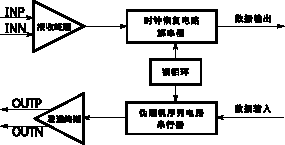
\includegraphics[width=10cm]{./img/serdes_phylayer_summery.pdf}
\caption{SerDes物理层框图}
\label{fig:serdes_phylayer_summery}
\end{figure}

最初的并行原始信号由模数转换器给出,经过组帧、编码及加扰后进入物理层,由并串转换器转换为串行码流通过发送端驱动输出到信道上。
接收端由信道经过输入捕获电路得到串行码流,时钟恢复电路通过信息码字的边沿获取时钟信号,并结合锁相环输出恢复出的时钟信号供接收端各模块使用。
收到的码流进入由恢复后的时钟信号驱动的串并转换器转换为最终的并行信号,输出至上一层逻辑,在经过解扰、解码及解帧后恢复出原始信号。

\subsubsection{时钟恢复电路}

时钟恢复电路是高速串行通信所必须具有的核心电路。
时钟恢复电路所需要做的就是根据参考时钟,从接收到的串行信号中将时钟信号提取处来。
在串行传输中,信道上只有串行数据在传输,并没有单独的可以同步的时钟信号。
这就需要接收端从信号中提取出时钟信号,以方便获取正确的码流。

时钟恢复电路主要实现两个基本功能,一是对数据信号的边沿进行监测,二是通过PLL产生稳定在输入数据流码率的输出信号,并且在信号缺少变化时保持自由振荡。
由此可见,在数据信道上传输的数据必须要有很高的随机性,能够保留足够多的边沿供时钟恢复电路恢复出时钟信号。
JESD204B通过对输入原始数据的编解码和加扰实现传输数据的随机性和均衡性,保证可提取边沿数量。
再通过接口握手时的码群同步,在连接建立初期使时钟恢复电路快速跟踪到当前信号的时钟频率。

\subsubsection{接收端和发送端电路}

为了确保端口的高速传输,SerDes的收发端驱动都是采用差分的CML电路。
典型的带锁存的差分CML电路如图\ref{fig:standard_CML_latch_with_poor_mirror_accuracy}所示。

\begin{figure}[H]
\centering
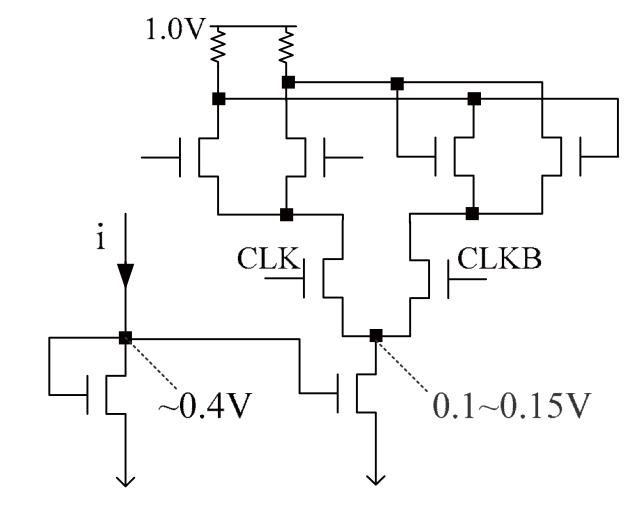
\includegraphics[width=8cm]{./img/standard_CML_latch_with_poor_mirror_accuracy.png}
\caption{典型的带锁存的差分CML电路}
\label{fig:standard_CML_latch_with_poor_mirror_accuracy}
\end{figure}

可以发现CML电路不同于传统的CMOS电路,该逻辑电路在上电时一直保持一定的电流通过,产生一定的功耗,而在高低电平转换时并不产生多余的电流损耗,这样即使在很高的传输速率下,收发端的功耗都保持在一个较低的水平。
CMOS电路在开通与关断时会产生能量损耗,在越高的传输的速率下,功耗越大。

相较于LVDS电路的并行传输,CML电路在引脚数量上有着明显的优势,在相同的通道数和模数转换分辨率前提下,CML电路引脚数量远小于CMOS电路和LVDS电路\cite{Harris2013}。
另外,CML电路采用差分传输,能够有效的抑制共模干扰,提高信号的信噪比,有理由更高速的传输。

\subsubsection{解串器和串行器}

解串器和串行器是SerDes收发端的核心功能电路。
解串器通过时钟恢复电路从信号中恢复得到的时钟,对输入码流进行串并转换,将串行信号恢复成并行信号,完成物理层的传输转化。
串行器通过锁相环生成的时钟信号,对输入的并行数据进行串行处理,最终得到输出码流,通过发送端CML电路发送至接收端。

解串器和串行器的工作速率也取决于自身的设计以及采用的电路逻辑.
受限于CMOS电路的工作频率,采用MCML电路的串并转换电路能够达到更高的切换速率。
但由于MCML电路需要保持一定的功耗,在低速情况下并没有优势,所以采用MCML电路作为解串器的第一级解串模块,作为串行器的最后一级串行模块,从而达到了速度和功耗的平衡\cite{tanabe20010}。

\subsection{半定制数字芯片设计流程介绍}

ASIC设计可以分为全定制设计以及半定制设计,其中半定制设计拥有设计周期短、设计成本低的优势。
虽然半定制设计相较于全定制设计缺乏一定的灵活性,但在针对一些特殊的应用设计有着一定的优势。
半定制设计方法其实是一种使用芯片厂方提供基本元件库的约束性设计,这样做的目的就是尽可能的简化设计\cite{yaoyf2006}。
在半定制设计中,对于基本门电路的设计细节不需要工程师再去考虑,只要选取合适的工艺库就可以达到预期的效果,这样的优势使半定制设计广泛运用于数字逻辑电路设计中。

ASIC半定制数字芯片设计的主要流程可以分为三大部分:系统级开发设计、RTL级开发设计和门级综合验证。

\subsubsection{系统级开发设计}

在系统及开发设计过程中主要是针对项目开发的需求,规划出合理的系统结构,分模块的设计整个系统。
在最初的系统结构设计中就需要规划好几个重要的功能模块,比如说输入输出端口模块、边界扫描逻辑模块、核心功能逻辑模块和锁相环时钟模块。
不同的设计需求可能由不同的核心模块,比如说强调实时处理的应用就需要在系统设计时考虑添加快速计算的模块。
在系统设计时还要考虑一些细节的问题,比如系统的复位布局,同步设计,跨时钟数据传输等。

总之,系统级开发设计是决定一个系统功能、性能及瓶颈的重要阶段,系统级设计的好坏直接关系到整个芯片的功能及稳定性。

\subsubsection{RTL级开发设计}

RTL级开发设计有些类似于FPGA的开发设计流程,需要针对每一个系统模块进行实现,这一过程多采用硬件描述语言对业务逻辑进行描述,例如Verilog、VHDL等\cite{xiecs2001}。
在完成代码编辑后,需要通过编译软件对代码进行调试,主要检查是否存在语法错误,确保代码能够正常运行。
之后是功能仿真,即通过仿真软件对业务逻辑进行测试,通过测试激励和所得出的测试结果可以判断软件逻辑上的问题,并对代码进行修改。
重复以上步骤,直到设计达到需求指标,能够实现预期功能。
在最后,由于可综合的代码和可仿真的代码是有一定区别的,一些语言的特性无法产生确定的硬件电路,这就需要在设计的时候有意识的采用可综合的逻辑进行描述,并在最后进行综合验证,确保设计结果能转换为标准逻辑单元。

RTL级的开发即为硬件设计的前端设计,重点就是使用硬件描述语言对应用逻辑进行描述并最后完成可综合的代码。
这一步骤决定了硬件设计中各个功能模块的正确性及稳定性。

\subsubsection{门级综合验证}

门级综合验证是ASIC设计过程的最后一步,这一步主要完成后续的门级综合和验证。
在RTL的综合过程中使用的是标准的理想逻辑器件,只是保证逻辑的正确性和可综合性,在门级综合步骤就涉及到了具体的厂方提供的工艺库。
不同厂家提供的工艺库是不同的,除了基本元器件有一定的区别,不同工艺在不同环境下的表现都是不相同的。
在门级综合验证的过程中就是将设计描述转换到厂家库的电路网表中。
在综合完成后就可以得到具体的设计运用单元数、面积、时序、功耗等信息。
另外还需要对综合结果进行时序分析、形式验证和布局布线,使整个芯片的规模布局达到所需要的要求。
最后输出的版图还需要对比逻辑图进行对比,并完成设计规则检查。

门级综合验证步骤是最接近硬件电路的阶段,整个芯片设计的成败也依赖于这一级别的设计。
重点就是对已经完成逻辑设计的代码进行转换,得到具体的电路,并针对电路进行仿真、修改、布局布线等工作,最终得到版图网表。

\subsection{设计工具介绍}

半定制数字逻辑电路设计有着一套完整的工具链,由几家著名的软件公司提供,如Synopsis、Cadence、Mentor Graphics等。
从代码编辑到编译综合,从模拟集成电路到数字集成电路,从逻辑验证到版图验证,从全定制设计到半定制设计,都有相应的软件支持。
大部分的电路设计工具由于需要牵涉到大量的数据运算,所以都选择安装在相对稳定高效的Linux平台。
并且为了保证设计的稳定性,一般都需要配置较高的电脑才能顺利运行响应软件,例如Cadence公司最新的IC616在64位系统环境下最低的配置要求即为8GB内存。

本文涉及到的设计工作,主要包括RTL级逻辑设计、编译、仿真和门级综合,所以使用了Mentor Graphics公司的Modelsim、SpringSoft公司的RTL级Debug工具Verdi3和Synopsis公司的门级综合工具Design Compiler。

\subsubsection{Verdi3}

Verdi3是SpringSoft公司推出的最新一代自动化IC设计侦错工具,具有很强的用户自定义功能,能够定制包括功能、环境以及增强工具在内的一系列功能\cite{lun2012}。
Verdi3在集成电路设计流程中主要负责Debug环节,它有两个重要作用,侦错和理解设计。
Verdi3平在较之前的产品,性能上有了大幅的提升,并提供了更加弹性化的工作环境定制。
Debug集成工具一个最重要的功能在于通仿真软件的兼容,以保证联调顺利,能够使硬件设计如同软件设计一样,在设计的同时快速的给出仿真结果,以便设计人员快速调试。
其中最重要的一部分就是对于通用的快速信号数据库(FSDB)的支持,Verdi3升级了快读信号数据库的访问速度,能够以多线程的方式读写并行逻辑仿真档案的输出\footnote{Parallel Logic Simulation Dumping}。
Modelsim的仿真结果可以以快速信号数据库的形式输出,这就使得两者之间实现了联调,便于测试和仿真。

\subsubsection{Modelsim}

Mentor Graphics公司的Modelsim一直以来是业界首选的硬件描述语言仿真人间,它提供了十分便捷的仿真环境,并且能够支持VHDL和Verilog语言的混合仿真\cite{fanj2010}。
Modelsim不仅能够进行仿真,还能很好的对仿真结果波形进行分析比较,并对程序代码进行调试,检测代码覆盖率。
Modelsim还能支持将输出各种格式的仿真结果,其中就包括快速信号数据库格式,这就保证了Modelsim能够和Verdi等其他Debug软件进行联合调试,各取所长。

尽管Modelsim也提供了调试功能,但相较于专门用于代码调试的Verdi平台,功能略显单薄。
而Verdi仅支持调试功能而不支持仿真功能,所以采用Modelsim提供的仿真结果文件进行分析,两者之间实现联调。

\subsubsection{Desgin Compiler}

Synposis公司的Design Compiler工具是一款优秀的逻辑综合工具,能够将抽象的RTL级代码综合为对应工艺库的门级网表。
Design Compiler提供了丰富的约束条件,来对设计进行约束,例如最大面积约束、输入延时约束、时钟约束等。
他主要通过三个步骤完成电路综合,第一步是是将RTL代码翻译成理想逻辑电路,第二步是在约束条件下将逻辑结构映射到具体工艺库上,第三步就是逻辑优化,具体可以分为架构级优化、逻辑级优化和门级优化,最终完成综合输出网表文件\cite{yangg2010}。
Desig Compiler支持自顶向下、自底向上和混合这三种综合策略,可以根据具体情况原则综合策略。
一般情况下,受限于计算机的运算能力,百万门以下级别的设计采用自顶向下的综合策略,百万门以上级别的设计则根据实际情况选择自底向上或者混合模式的综合策略。

综合完成后,Design Compiler能够通过工艺库的指标给出详细的综合结果,包括模块面积、线路面积、功耗、最大时延等项目,并且可以根据需求,由综合人员自行定制综合结果输出。

\bibliography{../../bib/serdes}
\end{document}
